\section{Deep Learning Results}\label{sec:dlresults}

The TinyCNN variants described in \cref{sec:network} are compared with the CNN site by evaluating the difference in their fidelities, expressed in percentage points (p.p.), where $\Delta \mathcal{F} = \mathcal{F}_{\text{TinyCNN}} - \mathcal{F}_{\text{CNN site}}$ and $\mathcal{F}$ denotes the fidelity defined in \cref{eq:fidelity}. A positive value indicates an improvement, corresponding to fewer errors than the CNN site, while a negative value indicates a higher error rate. One percentage point represents one percent of the test decisions being correct or incorrect. The simulated test set has 10\,809 decisions (1201 images with 9 sites each), so 1 p.p. corresponds to approximately 108 decisions, and a single incorrect decision represents \num{0.0093} p.p. The experimental test set contains 102\,718 decisions (406 images with 253 sites each), so 1 p.p. is approximately 1027 decisions, and one incorrect decision corresponds to \num{0.0010} p.p. These values are indicated in the figure legends.

\subsection{Simulated Data}

\begin{figure}[H]
    \centering
    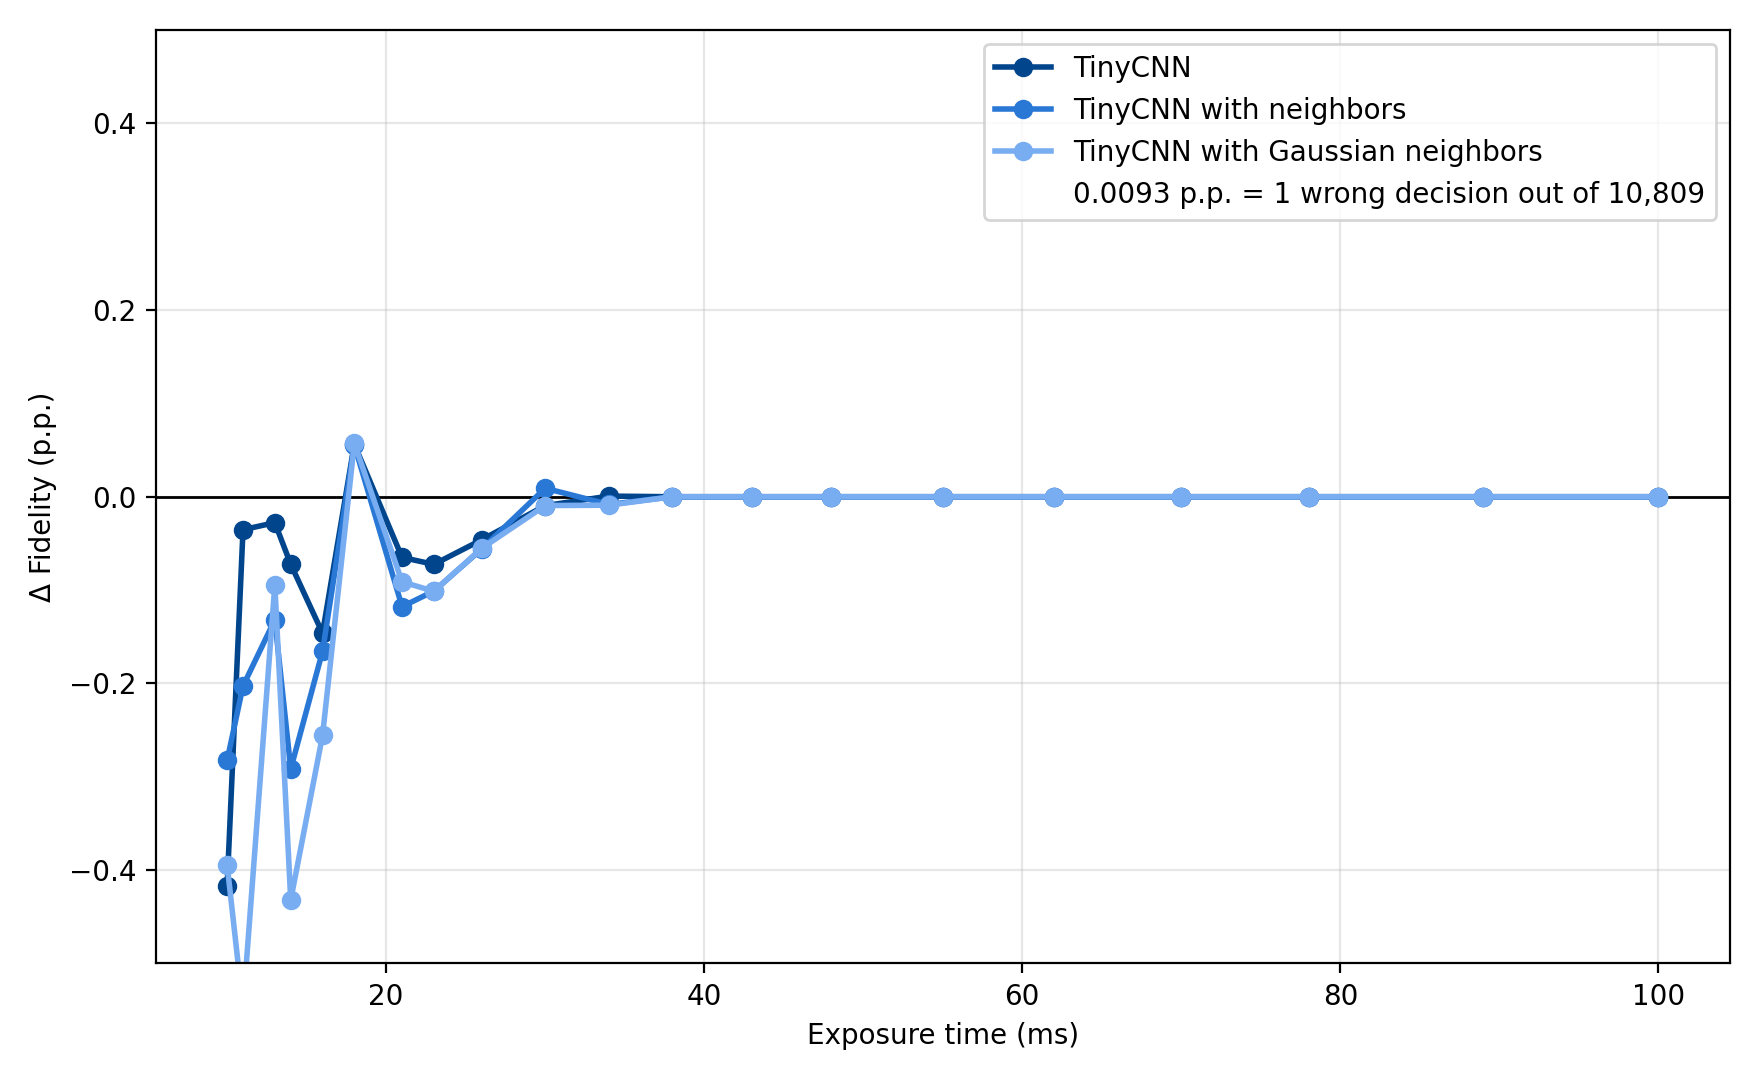
\includegraphics[width=0.85\textwidth]{fidelity_delta_from_cnn_site.png}
    \caption[Fidelity difference of the TinyCNN variants to the CNN site on the simulated data.]{Fidelity difference of the TinyCNN variants to the CNN site on the simulated data. Positive values are an improvement over the CNN site.}
    \label{fig:delta-sim}
\end{figure}

\Cref{fig:delta-sim} presents $\Delta \mathcal{F}$ as a function of exposure time. From \SI{38}{\milli\second} onward, $\Delta \mathcal{F}$ is zero for all variants. From \SI{30}{\milli\second} onward, the difference is at most one incorrect decision. At shorter exposure times, the differences remain small and fluctuate in sign. Up to \SI{26}{\milli\second}, the TinyCNN variants have a slightly higher error rate than the CNN site, averaging \num{0.09}\,p.p.\ for TinyCNN, \num{0.14}\,p.p.\ with neighbors, and \num{0.21}\,p.p.\ with Gaussian neighbors, with a maximum of \num{0.55}\,p.p., corresponding to approximately 59 decisions. Despite having approximately \SI{99}{\percent} fewer parameters than the CNN site, TinyCNN maintains the fidelity within a few tenths of a percentage point.

\subsection{Experimental Data and Model Selection}

\begin{figure}[H]
    \centering
    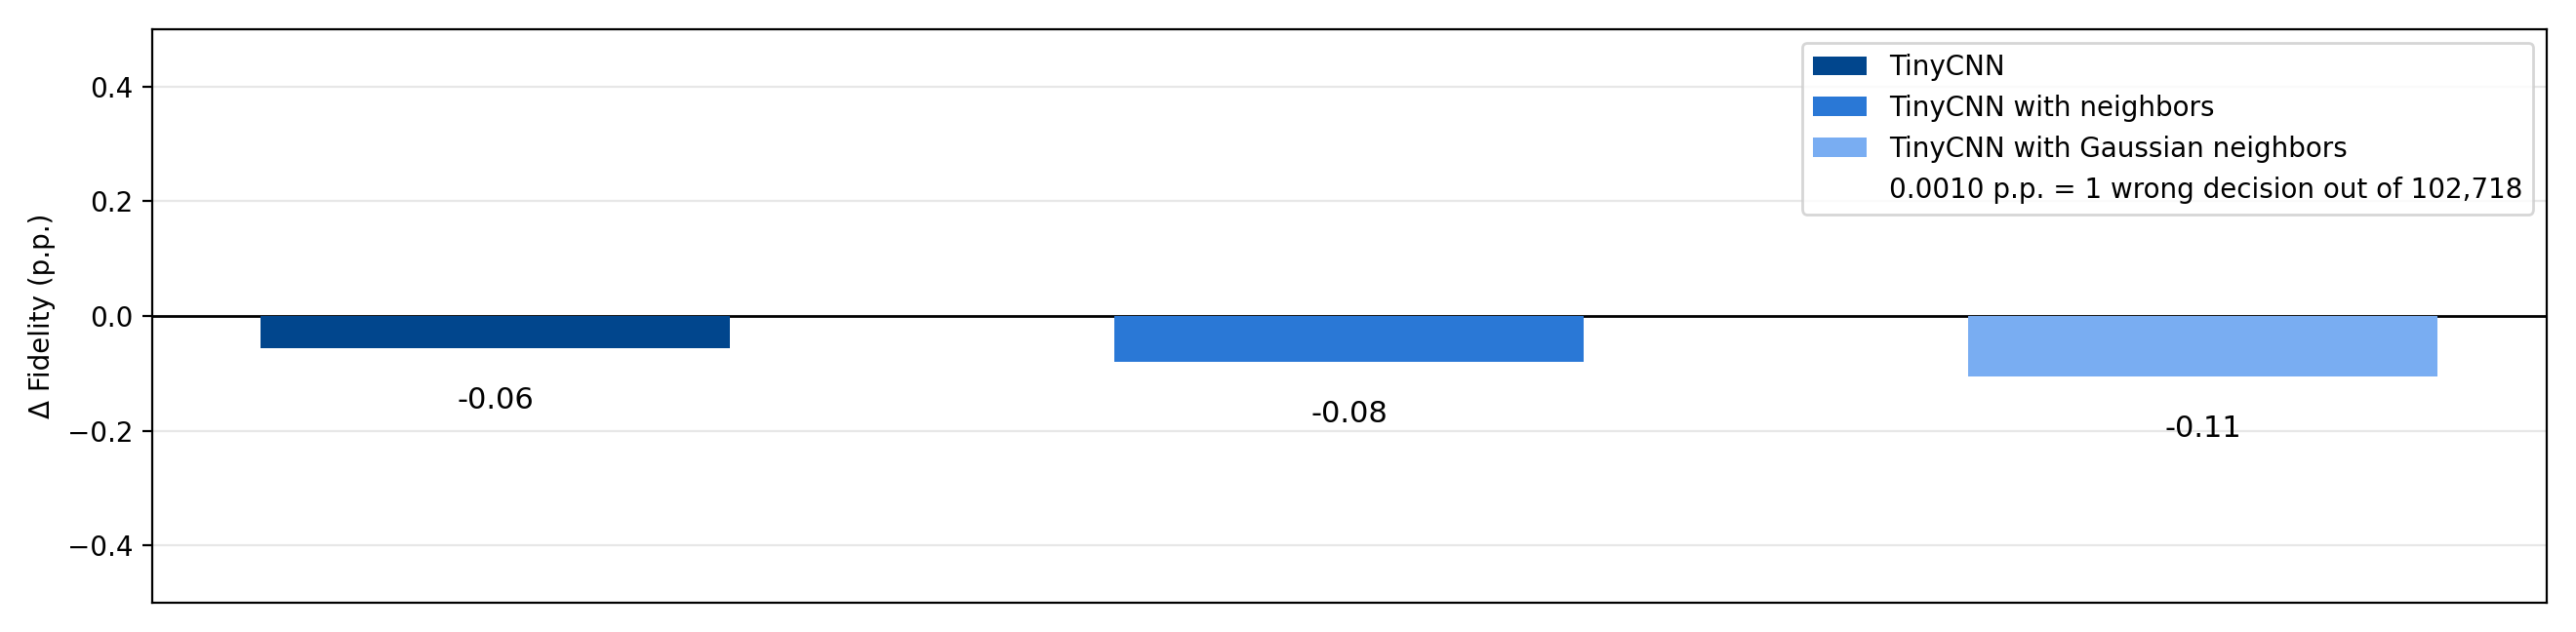
\includegraphics[width=1\textwidth]{real_dataset_vs_cnn_site.png}
    \caption[Fidelity difference of the TinyCNN variants to the CNN site on the experimental data.]{Fidelity difference of the TinyCNN variants to the CNN site on the experimental data. Positive values are an improvement over the CNN site.}
    \label{fig:delta-real}
\end{figure}

The experimental dataset consists of 2024 images of $600\times700$ pixels with 253 sites. In comparison with the simulation, the sites are farther apart, about 27 instead of 7 pixels, and the point-spread function is wider, with a width of 2.6 instead of 0.9 pixels. Therefore, the models are trained on $20\times20$ pixel crops instead of $10\times10$ pixel crops.
\Cref{fig:delta-real} shows that all three TinyCNN variants have a lower fidelity than the CNN site on the experimental data: by \num{0.06}\,p.p.\ for the TinyCNN, \num{0.08}\,p.p.\ with neighbors, and \num{0.11}\,p.p.\ with Gaussian neighbors. The differences between the variants are small, 21 to 45 errors out of about 1700, which is comparable to the fluctuation of an error count of this size, so the ordering may be noise.

\medskip
No variant is clearly best. On the experimental data, the TinyCNN without neighbors is nominally the closest to the CNN site, and in the simulation it is the best of the three at 8 of the 11 exposure times where the variants differ, against 2 for the neighbors and 1 for the Gaussian neighbors. The neighbor information therefore gives no measurable advantage at the spacings of these datasets. The TinyCNN with neighbors is used for the FPGA implementation because it has fewer parameters than the TinyCNN without neighbors, and because the mean of a crop requires only additions, whereas the Gaussian-weighted mean requires a multiplication for each pixel. The variants share the loss, optimizer, and data split procedure; the maximum training budget and early stopping settings are listed in Appendix~\ref{app:training}.